%\documentclass[12pt,serif]{beamer}
%\documentclass[tikz,12pt,svgnames]{beamer}
\documentclass[table,handout,tikz,12pt,svgnames]{beamer}
\usepackage{CM-preamble}
\subtitle{\Huge Recursivité}
\date{CM4}

%README TODO STUFF
%README This presentation is not as well made as previous ones. For example, pseudo code is not underlined and some things are not well aligned.

\begin{document}

\begin{frame}
	\titlepage
\end{frame}

\begin{frame}[fragile=singleslide]
	\frametitle{La récursivité: Liste chaînée}
%\vspace{-0.7cm}
\begin{center} \noindent\makebox[\linewidth]{
\begin{tikzpicture}
%%\foreach \index/\list in {1/{a,b,null}, 2/{c,null}, 3/{d,null}} {
\foreach \index/\list in {1/{$a_0$,$a_2$,$a_3$,$a_4$}} {
	\node[array element] (aux) at (0,-\index) {L};
    \LinkedList{\list}
}
\node at (2.5,-2) {\texttt{<elt>}};
\draw[dash pattern=on 6pt off 3pt, line width = 0.7mm] (3.5,-0.2) -- (3.5,-2.4) ;
\node at (6.5,-2) {\texttt{<liste>}};
\draw[dash pattern=on 6pt off 3pt, line width = 0.7mm] (9.65,-0.2) -- (9.65,-2.4) ;
\node at (10.2,-2) {\texttt{$\emptyset$}};

%\draw[<->] ([shift={(0,-1)}]-1,-1) --  ([shift={(-2,-2)}]4.2,-1);
%\draw[<->] ([shift={(0.5,0.5)}]4.4,-1) --node[below] {Zone d'extension contigue} ([shift={(0.5,0.5)}]9.6,-1);

\end{tikzpicture}
}
\end{center}
	\vspace{-0.9cm}
		\begin{block}{} %Gestion dynamique de la mémoire}
			\begin{itemize}
			\item Structure de données récursive :\\
			\texttt{<liste> ::= <elt> <liste> | $\emptyset$ }
			\end{itemize}
		\end{block}
	  \begin{columns}[c]
  		\hspace{-0.5cm}
	  	\begin{column}{0.7\textwidth}
		\begin{block}{Déclaration} %Gestion dynamique de la mémoire}
			\begin{minted}[mathescape=true,escapeinside=||,tabsize=4,fontsize=\footnotesize,]{c}
	type Liste = pointeur de Cellule
	type Cellule = structure
		 valeur : <T>
		 suivant : Liste
	fin
			\end{minted}
		\end{block}
		\end{column}
%		\setlength{\columnseprule}{0.4pt}
		\hspace{-1.3cm}
		\vrule{}
		\hspace{0.3cm}
		\begin{column}{0.38\textwidth}
		Récursivité croisée	(ou indirecte)
	    \end{column}
	\end{columns}
\end{frame}


\begin{frame}[fragile=singleslide]
	\frametitle{La récursivité}
		\vspace{-0.8cm}
		\begin{block}{} %Gestion dynamique de la mémoire}
			\begin{itemize}
				\item Une entité (SD, algorithme) est récursive si elle se définit à partir d'elle
				même
				\item Algorithmes récursifs (exemple : factorielle, fibonacci)
				%\begin{itemize}
				\vspace{0.3cm}
				\begin{block}{Exemple d'algo récursive: Factorielle}
					\item Analyse récurrente
					\begin{itemize}
						\item $ n! = n * (n-1)!$
						\item $ 0! = 1 $
					\end{itemize}
				\vspace{0.5cm}
				\hspace{-2cm}
				\item Écriture fonctionnelle
				\begin{columns}[b]
				  	\hspace{-0.3cm}
				  	\begin{column}{0.55\textwidth}
						\begin{itemize}
							\item \texttt{fact(n) = n * fact(n-1)}
						\end{itemize}
					\end{column}
			%		\setlength{\columnseprule}{0.4pt}
					\hspace{-0.3cm}
					\vrule{}
					\hspace{0cm}
					\begin{column}{0.45\textwidth}
						\begin{itemize}
							\item Cas général, récursif
						\end{itemize}
				    \end{column}
				\end{columns}
				\begin{columns}[c]
				  	\hspace{-0.3cm}
				  	\begin{column}{0.55\textwidth}
						\begin{itemize}
							\item \texttt{fact(0) = 1}
						\end{itemize}
					\end{column}
			%		\setlength{\columnseprule}{0.4pt}
					\hspace{-0.3cm}
					\vrule{}
					\hspace{0cm}
%					\vspace{5cm}
					\begin{column}{0.45\textwidth}
						\begin{itemize}
							\item Cas primitif, terminal
						\end{itemize}
				    \end{column}
				\end{columns}
				\end{block}
				%\end{itemize}
			\end{itemize}
		\end{block}
\end{frame}

\begin{frame}[fragile=singleslide]
	\frametitle{Factorielle}
%		\vspace{-0.8cm}
				\begin{columns}[T]
				  	\hspace{-0.3cm}
				  	\begin{column}{0.5\textwidth}
				  	\begin{block}{Algorithme}
						\begin{minted}[mathescape=true,escapeinside=||,tabsize=3]{c}
fonction fact(n) : entier
	D : n : entier
	L : f : entier
	si n = 0 alors
		f |$\leftarrow$| 1
	sinon
		f |$\leftarrow$| n * fact(n­1)
	fsi
	retourner(f)
ffonction
						\end{minted}
					\end{block}
					\end{column}
			%		\setlength{\columnseprule}{0.4pt}
%					\hspace{-0.25cm}
					\vrule{}
%					\hspace{0cm}
%					\vspace{5cm}
				  	\begin{column}{0.55\textwidth}
				  	\begin{block}{Fonction en C}
						\begin{minted}[mathescape=true,escapeinside=||,tabsize=3]{c}
int fact (int n) {
	if (n==0)
		return 1;
	else
		return(n * fact(n-1));
}
						\end{minted}
					\end{block}
					\end{column}
				\end{columns}
\end{frame}

\begin{frame}[fragile=singleslide]
	\frametitle{Exemple d'exécution d'une factorielle}
	{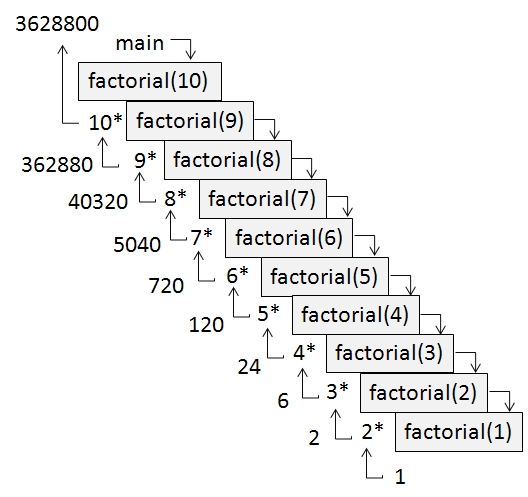
\includegraphics[scale=0.50]{../common-images/RecursiveFactorial.jpg}}
\end{frame}

\begin{frame}[fragile=singleslide]
	\frametitle{Conception récursive d'algorithmes}
	\begin{block}{3 parties} %Gestion dynamique de la mémoire}
		\begin{itemize}
			\item \textbf{Cas généraux récursifs:} \\ Résolution du problème par lui même
			\item \textbf{Cas terminaux non récursifs:} \\ Résolution immédiate du problème)
			\item \textbf{Conditions de terminaison}
		\end{itemize}
	\end{block}
\end{frame}

\begin{frame}[fragile=singleslide]
	\frametitle{Exemple : Suite de Fibonacci}
	\begin{minted}[mathescape=true,escapeinside=||,tabsize=4]{c}
	\end{minted}
\end{frame}




\begin{frame}[fragile=singleslide]
	\frametitle{Recherche dichotomique dans une liste contiguë: trouver l'élément \texttt{x}}

	\begin{block}{}
	\vspace{-0.4cm}
	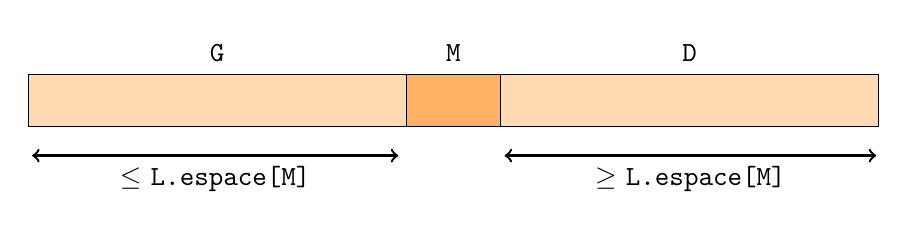
\begin{tikzpicture}
	% size of each node
	\def\sz{6.5mm}
	\def\szwidth{12mm}
	\def\offset{0.6}
	% node style definition
	\tikzstyle{block} = [draw, fill=orange!30, rectangle, minimum height=\sz, minimum width=\sz ];
	\tikzstyle{rect} = [draw, fill=orange!60, rectangle, minimum height=\sz, minimum width=\szwidth ];
	\tikzstyle{rect2} = [draw, fill=orange!30, rectangle, minimum height=\sz, minimum width=\szwidth*4 ];
	\tikzstyle{indices} = [rectangle, minimum height=\sz, minimum width=\szwidth ];
	\tikzstyle{plain} = [draw=none,fill=none];
	% array element definition
%	\def\dateone{$A_0$,\ldots \ldots,$A_n$,,};
%	\def\datetwo{0,,dernier,,MAX-1};
	%\def\x{0}; % x pos of arr
	%\def\y{0}; % y pos of arr
	\newcounter{ind};
	\setcounter{ind}{0};
%	\node[plain] { x };
%	\node[rect] (first) at (0*\szwidth,\offset) { };
	\node[rect2] at (0,\offset) { };
	\node[rect] (middle) at (2.5*\szwidth,\offset) { };
	\node[rect2] at (5*\szwidth,\offset) { };
%	\node[rect] (last) at (8*\szwidth,\offset) {  };
	\node[indices] at (0*\szwidth,2*\offset) { \texttt{G} };
%	\node[indices] at (2*\szwidth,0) {  };
	\node[indices] at (2.5*\szwidth,2*\offset) { \texttt{M} };
%	\node[indices] at (6*\szwidth,0) {  };
	\node[indices] at (5*\szwidth,2*\offset) { \texttt{D} };
%	\foreach \item in \dateone {
%		\addtocounter{ind}{1};
%		\node[block] at (\theind*\sz,0) { \item };
%		\node[rect] at (\theind*\szwidth,1.7) { \item };
%		\node[rect] at (\theind*\szwidth,\offset) { \item };
%	}
%	\draw[<->]([yshift=-3mm]dateone-2.south west) -- node[below] {Tableau de longeur 10} ([yshift=-3mm]dateone-2.south east);
%	\draw[<->]([yshift=-3mm ]) -- node[below] {Tableau de longeur 10};
%	\draw[<->]([yshift=-8mm]first.south) edge ([yshift=-8mm]middle.south);
%	\draw[<->]([yshift=-8mm]last.south) edge ([yshift=-8mm]middle.south);
	\draw[<->,line width = 0.3mm] (-2.35,-0.1) -- node[below] {$\le$ \texttt{L.espace[M]}} (2.3,-0.1);
	\draw[<->,line width = 0.3mm](3.65,-0.1) --node[below] {$\ge$ \texttt{L.espace[M]}} (8.37,-0.1);

	\setcounter{ind}{0};
	%\node[plain] at (0,\offset) { d1 };
%	\foreach \item in \datetwo {
%		\addtocounter{ind}{1};
%		\node[indices] at (\theind*\szwidth,0) { \item };
%	}
	\end{tikzpicture}
	\vspace{-1cm}
	\end{block}
	\begin{block}{}
		\begin{itemize}
			\item Dichotomie sur \texttt{L.espace}
			\item \textbf{Cas général:} \texttt{X $\ne$ L.espace[M]}  $\Rightarrow$ dichotomie à gauche ou à droite
			\item \textbf{Cas terminal :} \texttt{X = L.espace[M]}
			\item \textbf{Condition de terminaison :} \texttt{G > D} (non trouvé)
		\end{itemize}
	\end{block}
\end{frame}


\begin{frame}[fragile=singleslide]
	\frametitle{Recherche dichotomique: liste contiguë}
	\vspace{-0.15cm}
	\begin{minted}[mathescape=true,escapeinside=||,tabsize=3,		fontsize=\footnotesize]{text}
|\underline{Action}| Dichotomie(L,X,G,D,pos,existe)
	|\underline{D}| : L : liste contiguë d'entiers
	    X, G, D : entier
	|\underline{R}| : pos: entier ; existe : booléen
	|\underline{L}| : M : entier
	|\underline{Si}| G>D |\underline{Alors}|
		existe |$\leftarrow$| faux
	|\underline{Sinon}|
		M |$\leftarrow$| (G + D) / 2
		|\underline{Si}| X = L.espace[M] |\underline{Alors}|
			existe |$\leftarrow$| vrai
			pos |$\leftarrow$| M
		|\underline{Sinon}|
			|\underline{Si}| X < L.espace[M] |\underline{Alors}|
				dichotomie(L,X,G,M-1,pos,existe)
			|\underline{Sinon}|
				dichotomie(L,X,M+1,D,pos,existe)
			|\underline{Fsi}|
		|\underline{Fsi}|
	|\underline{Fsi}|
|\underline{Faction}|
	\end{minted}
\end{frame}

\begin{frame}[fragile=singleslide]
	\frametitle{Récursivité sur les listes}
%	\frametitle{HARD SLIDE}
	\begin{block}{SD récursives $\Rightarrow$ algorithmes récursifs} %Gestion dynamique de la mémoire}
		\begin{itemize}
			\item \texttt{<liste> ::= $\emptyset$	|	<elt> <liste>} \\
			\vspace{0.5cm}

			où :
			\begin{itemize}
			\item $\emptyset$ $\rightarrow$ cas terminal
			\item \texttt{<elt>} $\rightarrow$ traitement de l'élément (éventuellement cas terminal)
			\item \texttt{<liste>} $\rightarrow$ traitement récursif (cas général)
			\end{itemize}
		\end{itemize}
	\end{block}
\end{frame}

\begin{frame}[fragile=singleslide]
	\frametitle{Récursivité sur les listes}
%	\vspace{-0.8cm}
	\begin{block}{Longueur d'une liste} %Gestion dynamique de la mémoire}
		\begin{itemize}
			\item \texttt{L = <elt> <liste>} \\ \texttt{longueur(L) = 1 + longueur(L$\uparrow\bullet$suivant)}
			\item \texttt{L = $\emptyset$} \\ \texttt{longueur(L) = 0}
		\end{itemize}
	\end{block}
	\begin{block}{Algorithme} %Gestion dynamique de la mémoire}
		\begin{minted}[mathescape=true,escapeinside=||,tabsize=3,fontsize=\small]{text}
fonction longueur (L) : entier
	D : L : liste
	Si L = NULL Alors
		retourner(0)
	Sinon
		retourner(1 + longueur(L|$\uparrow\bullet$|suivant))
	Fsi
ffonction
		\end{minted}
	\end{block}
\end{frame}


\begin{frame}[fragile=singleslide]
	\frametitle{La récursivité : \texttt{inverser()} récursive}
%	\vspace{-0.8cm}
	\begin{block}{Inverser une suite de caractères} %Gestion dynamique de la mémoire}
		\begin{itemize}
			\item $s=<c_1, c_2, \ldots, c_n, \bullet >$ : \texttt{inverser} $<c_n, \ldots, c_2, c_1>$
			\item cas généraux et terminaux ? conditions de terminaison ?
		\end{itemize}
	\end{block}
	\begin{block}{Algorithme} %Gestion dynamique de la mémoire}
		\begin{minted}[mathescape=true,escapeinside=||,tabsize=3,fontsize=\small]{text}
	Action inverser()
		L : c : caractère
		lire(c)
		Si c |$\ne$| '|$\bullet$|' Alors
			inverser()
			écrire(c)
		Fsi
	Faction
		\end{minted}
	\end{block}
\end{frame}

\begin{frame}[fragile=singleslide]
	\frametitle{La récursivité : \texttt{inverser()} itérative}
	\vspace{-0.8cm}
	\begin{block}{}
		\begin{itemize}
			\item mémoriser les caractères lus séquentiellement
			\item les restituer en ordre inverse de leur mémorisation
			\item $\Rightarrow$ mémorisation en pile
		\end{itemize}
	\end{block}
	\begin{block}{Algorithme} %Gestion dynamique de la mémoire}
		\begin{minted}[mathescape=true,escapeinside=||,tabsize=3,fontsize=\small]{text}
	Action inverser()
		L: c : caractère, P : Pile de caractères
		lire(c)
		TQ c |$\ne$| '|$\bullet$|'
			Faire empiler(P, c); lire(c);
		Fait
		{restituer en ordre inverse}
		TQ non pileVide(P) Faire
			dépiler(P,c) ; écrire(c);
		Fait
	Faction
		\end{minted}
	\end{block}
\end{frame}


\begin{frame}[fragile=singleslide]
	\frametitle{La récursivité : pile d'exécution d'un langage}
	\vspace{-0.2cm}
	\begin{block}{}
		\begin{itemize}
			\item Mémorise le contexte appelant lors d'un appel de fonction
			\item Restitue ce contexte lors du retour
			%\item $\Rightarrow$ mémorisation en pile
		\end{itemize}
	\end{block}
	\begin{block}{Exemple} %Gestion dynamique de la mémoire}
		\begin{minted}[mathescape=true,escapeinside=||,tabsize=3,fontsize=\small]{c}
void inverse(){
	char c;
	c = getchar();
	if (c != '.') {
		inverse() ; putchar(c);
	}
}
		\end{minted}
	\end{block}
\end{frame}

\begin{frame}[fragile=singleslide]
	\frametitle{La récursivité : pile d'exécution d'un langage}
	\vspace{-4cm}
	\begin{block}{Schéma d'exécution}
	\end{block}
\end{frame}

\begin{frame}[fragile=singleslide]
	\frametitle{La récursivité : conséquences}
	\vspace{-0.2cm}
	\begin{block}{}
		\begin{itemize}
			\item Fournit une méthode pour traduire itérativement (à l'aide d'une pile) des
			algorithmes récursifs = la dérécursivisation
			\item Récursivité $\Rightarrow$ surcoût dû à la pile
			\begin{itemize}
				\item exemple : dichotomie, factorielle, longueur
				\item contre-­exemple : inverser (en général pour une récursivité non terminale)
			\end{itemize}
			\item Intérêt général quand elle facilite l'analyse algorithmique d'un problème (récursif par nature; ex : SD récursive)
			\item Intérêt pour la parallélisation des tâches
		\end{itemize}
	\end{block}
\end{frame}

\begin{frame}[fragile=singleslide]
	\frametitle{La récursivité : insertion liste ordonnée}
%	\vspace{-0.2cm}
	\begin{block}{Insertion de x dans une liste ordonnée}
		\begin{itemize}
			\item \texttt{L = $\emptyset \Rightarrow$ L = <x>}
			\item \texttt{L = <elt> <L'>}
			\begin{itemize}
				\item \texttt{x $\le$ <elt> $\Rightarrow$ L = <x, elt> <L'>}
				\item \texttt{x $>$ <elt> $\Rightarrow$ insérer x dans <L'>}
			\end{itemize}
		\end{itemize}
	\end{block}
\end{frame}

\begin{frame}[fragile=singleslide]
	\frametitle{La récursivité : insertion liste ordonnée}
%	\vspace{-0.2cm}
	\begin{block}{} %Gestion dynamique de la mémoire}
		\begin{minted}[mathescape=true,escapeinside=||,tabsize=4,fontsize=\small]{c}
Action insérer(L, x)
	D/R : L : liste de <T>
	D : x : <T>
	Si L = |$\emptyset$| Alors
		ajoutTête(L, x)
	Sinon
		Si x |$\le$| L|$\uparrow\bullet$|valeur Alors
			ajoutTête (L, x)
		Sinon
			insérer(L|$\uparrow\bullet$|suivant, x)
		Fsi
	Fsi
Faction
		\end{minted}
	\end{block}
\end{frame}

%TODO: VERIFY CODE IN ELSE &(pl)>suivant,x.
%TODO: Also verify malloc, used to be allouer(&pt);
\begin{frame}[fragile=singleslide]
	\frametitle{La récursivité : insertion liste ordonnée}
%	\vspace{-0.2cm}
	\begin{block}{} %Gestion dynamique de la mémoire}
		\begin{minted}[mathescape=true,tabsize=4,fontsize=\small, linenos]{c}
void inserer(liste *pL, int x){
	if ( (*pL == NULL) || (x <= (*pL)->valeur) )
		 ajoutTête(pL, x);
	else
		inserer( &(*pL)->suivant, x);
}

void ajoutTête(liste *pL, int x){
	Ptcellule pt;
	pt = malloc(*pt);
	pt->valeur = x;
	pt->suivant = *pL;
	*pL = pt;
}
		\end{minted}
	\end{block}
\end{frame}

\begin{frame}[fragile=singleslide]
	\frametitle{La récursivité : insertion liste ordonnée}
	\vspace{-4cm}
	\begin{block}{Schéma d'exécution}
	\end{block}
\end{frame}


% % % % % % % % % % % % % % % % % % % % % % % % % % %
% END
% % % % % % % % % % % % % % % % % % % % % % % % % % %
\end{document}


% % % % % % % % % % % % % % % % % % % % % % % % % % %
% END
% % % % % % % % % % % % % % % % % % % % % % % % % % %

	\vspace{-0.9cm} \begin{center} \noindent\makebox[\linewidth]{\line(2,0){500}} \end{center}  \vspace{-0.7cm}
	\vspace{-0.9cm} \begin{center} \noindent\makebox[\linewidth]{\rule{\paperwidth}{1.5pt}}  \end{center}  \vspace{-0.7cm}
